\documentclass[border=4pt]{standalone}
\usepackage{tikz}
\usepackage{pgfplots}
\pgfplotsset{compat=1.18}
\usetikzlibrary{shapes.geometric,arrows.meta,positioning,calc,fit,decorations.pathreplacing,backgrounds}
\definecolor{boxblue}{RGB}{225,238,252}
\definecolor{boxgreen}{RGB}{225,247,231}
\definecolor{boxorange}{RGB}{253,236,216}
\definecolor{boxgray}{RGB}{237,237,237}
\definecolor{boxred}{RGB}{253,226,226}
\begin{document}
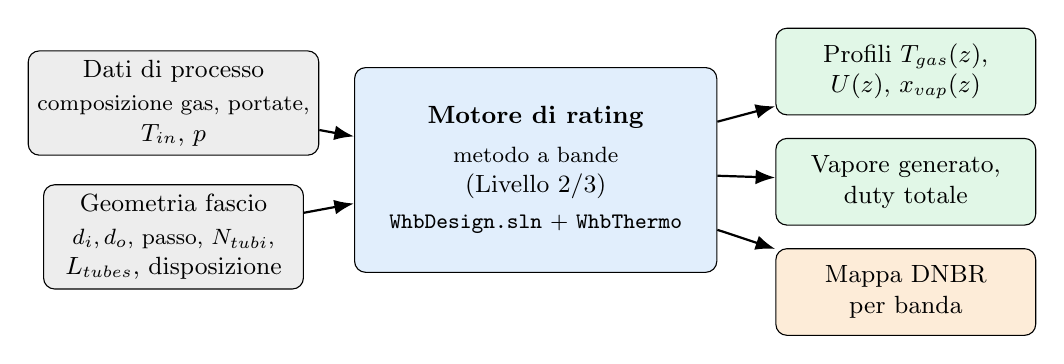
\begin{tikzpicture}[
  box/.style={draw, rectangle, rounded corners, minimum height=1.1cm, minimum width=3.3cm, align=center, font=\small},
  arr/.style={-{Latex[length=2.5mm]}, thick}
]
\node[box, fill=boxgray] (proc) at (0,0) {Dati di processo\\[1pt]\footnotesize composizione gas, portate,\\ $T_{in}$, $p$};
\node[box, fill=boxgray] (geo) at (0,-1.7) {Geometria fascio\\[1pt]\footnotesize $d_i,d_o$, passo, $N_{tubi}$,\\ $L_{tubes}$, disposizione};

\node[box, fill=boxblue, minimum width=4.6cm, minimum height=2.6cm] (core) at (4.6,-0.85) {\textbf{Motore di rating}\\[3pt]\footnotesize metodo a bande\\ (Livello 2/3)\\[2pt]\footnotesize \texttt{WhbDesign.sln} + \texttt{WhbThermo}};

\node[box, fill=boxgreen] (out1) at (9.3,0.4) {Profili $T_{gas}(z)$,\\ $U(z)$, $x_{vap}(z)$};
\node[box, fill=boxgreen] (out2) at (9.3,-1) {Vapore generato,\\ duty totale};
\node[box, fill=boxorange] (out3) at (9.3,-2.4) {Mappa DNBR\\ per banda};

\draw[arr] (proc) -- (core);
\draw[arr] (geo) -- (core);
\draw[arr] (core) -- (out1);
\draw[arr] (core) -- (out2);
\draw[arr] (core) -- (out3);
\end{tikzpicture}
\end{document}
